\chapter{Specyfikacja zewnętrzna}
\label{ch:04}

\section{Opis Aplikacji}

Aplikacja została stworzona w środowisku Unity i zapewnia interaktywną symulację rozprzestrzeniania się zarażeń w przestrzeni biurowej. Pozwala na zmianę wielu parametrów wpływających na przebieg symulacji. Ma na celu w prosty i zrozumiały dla każdego sposób pokazywać rozprzestrzenianie się choroby. Przeznaczona jest głównie dla użytkowników korzystających z komputerów osobistych z systemem operacyjnym Windows.

\section{Wymagania Sprzętowe}

\begin{itemize}
	\item Komputer z systemem operacyjnym Windows.
	\item Ekran o rozdzielczości co najmniej 1280x720 pikseli.
	\item Karta graficzna wspierająca OpenGL 3.2 lub nowszy.
\end{itemize}

\section{Wymagania Programowe}

\begin{itemize}
	\item System operacyjny: Windows 7/8/10 i nowsze.
	\item Zainstalowany runtime Unity w wersji zgodnej z aplikacją.
\end{itemize}

\section{Obsługa Aplikacji}

Do obsługi aplikacji wystarczy myszka, która umożliwia interakcję z interfejsem graficznym. Aplikacja nie wymaga dodatkowego sprzętu.
\begin{itemize}
	\item \textbf{Ustawianie Parametrów Symulacji}\\
			odbywa się poprzez wybranie odpowiednich wartości na suwakach.
	\item \textbf{Rozpoczęcie symulacji i jej kontrola}\\
			aby rozpocząć symulacje należy po ustawieniu parametrów wcisnąć przycisk start. W trakcie trwania symulacji jej prędkość można ustawiać odpowiednim suwakiem. Aby zatrzymać symulację należy wcisnąć przycisk pauzy. Aby zrestartować symulację należy wcisnąć przycisk restartu.
\end{itemize}

\section{Uruchamianie Aplikacji}

Aby skorzystać z aplikacji, należy wykonać poniższe kroki:

\begin{enumerate}
	\item Pobrać folder zawierający aplikację.
	\item Rozpakować pobrany folder w wybranym miejscu na dysku.
	\item Kliknąć w folder aplikacji.
	\item Kliknąć dwukrotnie plik wykonywalny (exe) aplikacji.
\end{enumerate}

Aplikacja uruchomi się bez konieczności instalacji.

\begin{figure}[h!]
	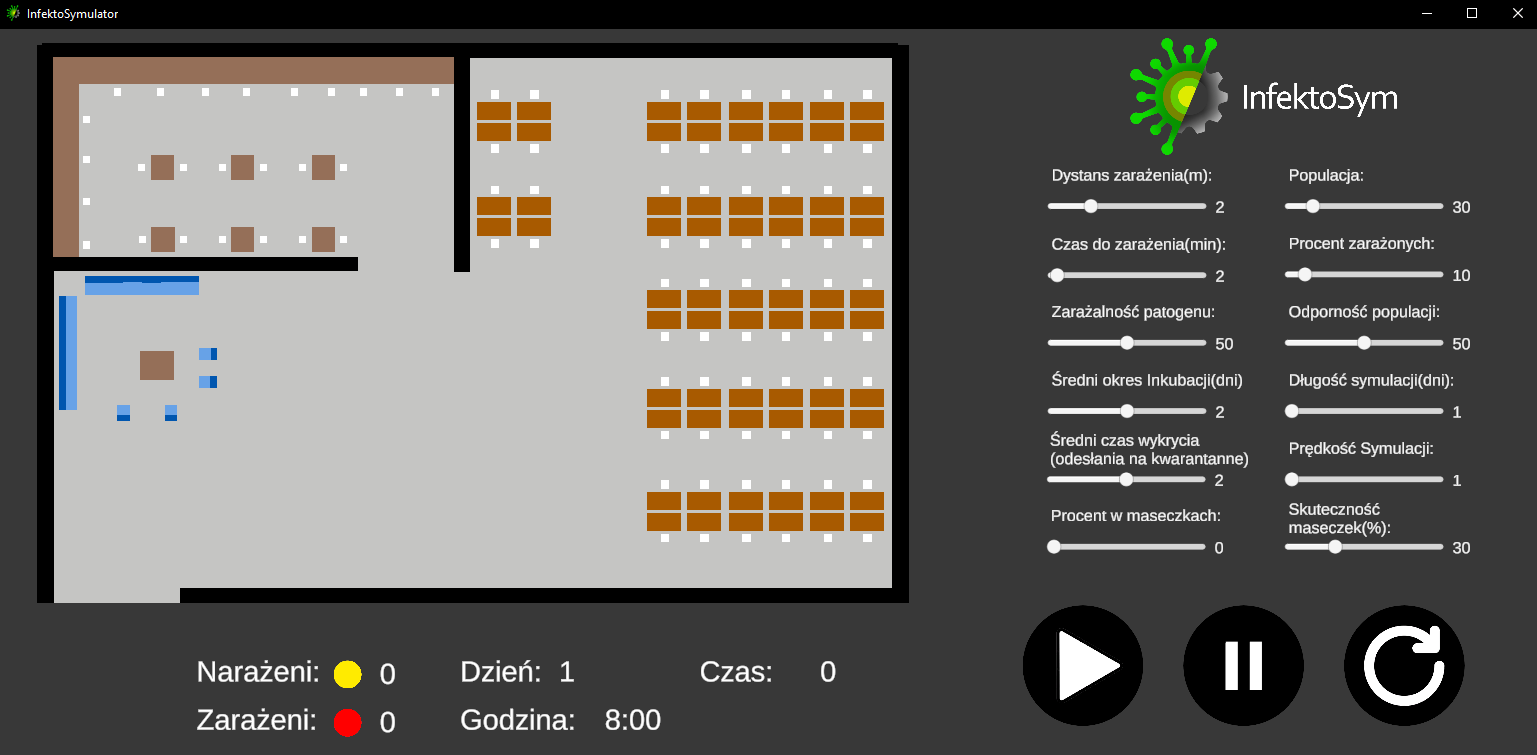
\includegraphics[width=\linewidth]{beforeSim.png}
	\caption{Ekran początkowy aplikacji.}
\end{figure}

\begin{figure}[h!]
	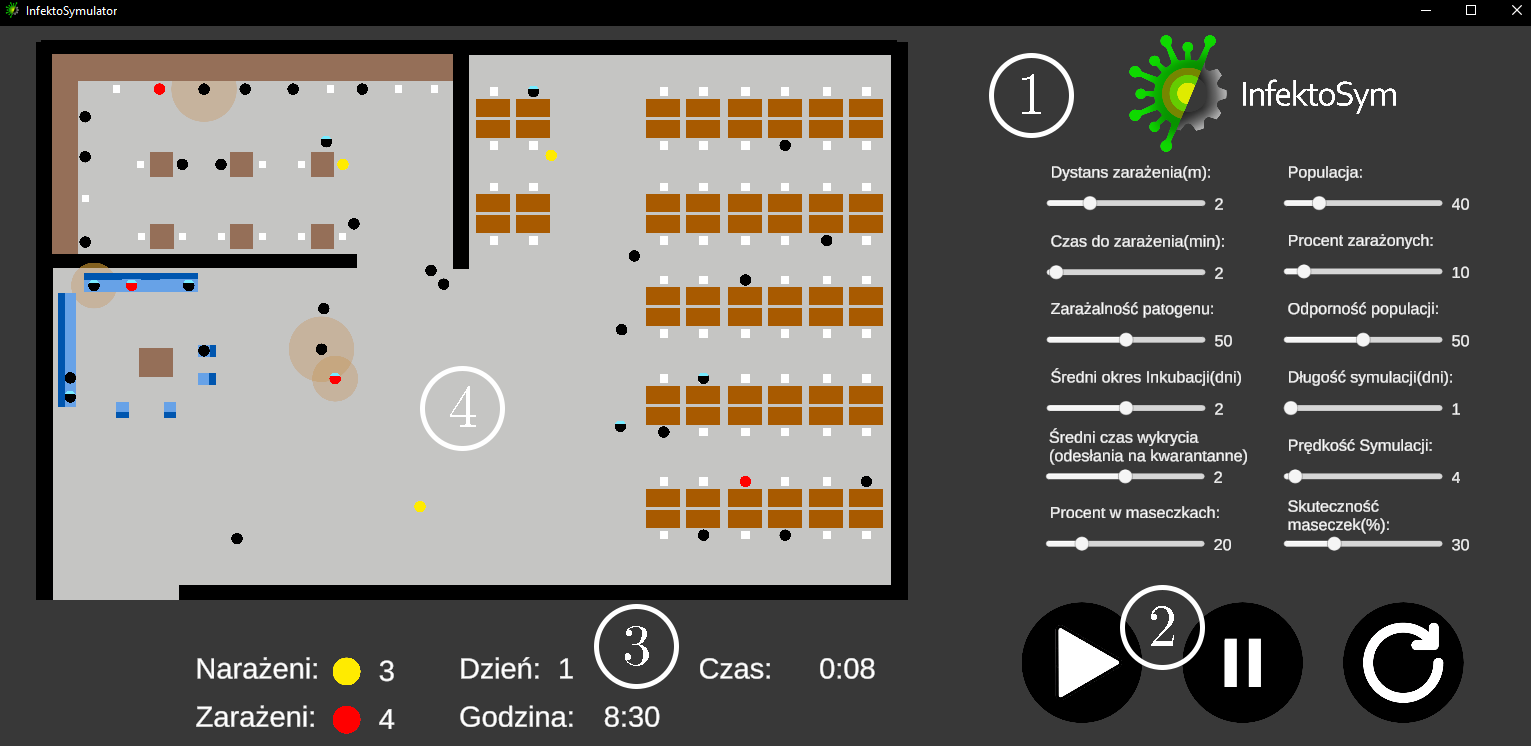
\includegraphics[width=\linewidth]{runningSimwithNumbers.png}
	\caption{Ekran podczas działającej symulacji: 1. Suwaki do ustawiania parametrów, 2. Przyciski kontrolujące 3. Aktualne statystyki i czas, 4. Wizualizacja}
\end{figure}

\begin{figure}[h!]
	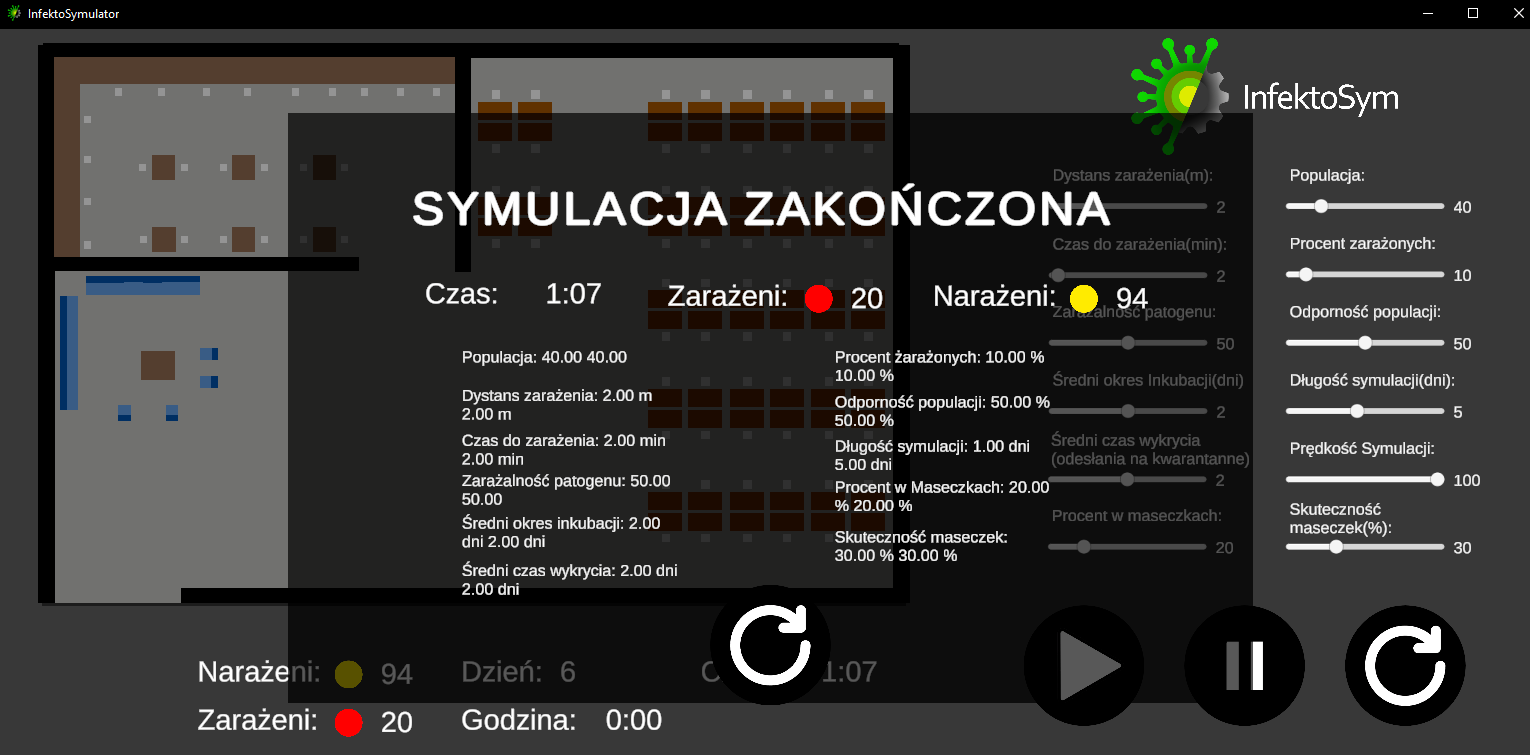
\includegraphics[width=\linewidth]{endSim.png}
	\caption{Ekran zakończenia symulacji}
\end{figure}

\begin{figure}[h!]
	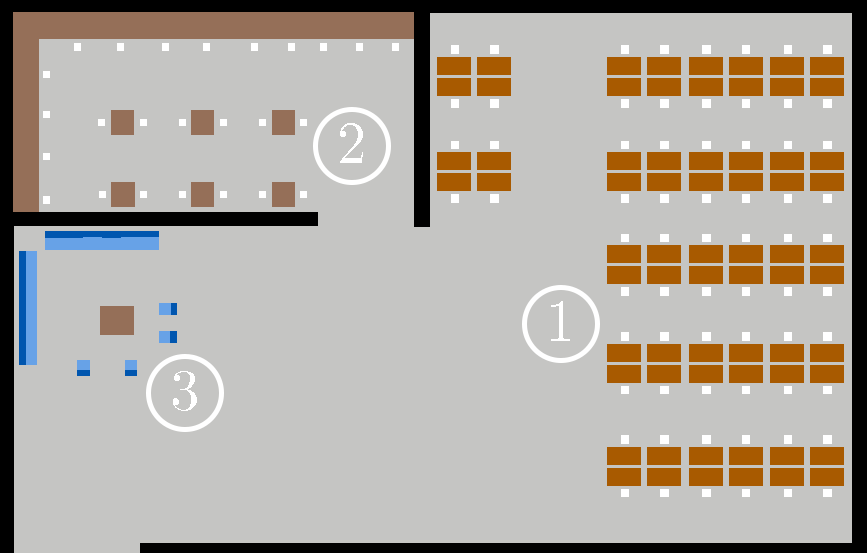
\includegraphics[width=\linewidth]{mapWithNumbers.png}
	\caption{Mapa biura: 1. Biurka do pracy, 2. Kuchnia ze stolikami, 3. Miejsce wypoczynku}
\end{figure}


%%%%%%%%%%%%%%%%%%%%%
%% RYSUNEK Z PLIKU
%
%\begin{figure}
%\centering
%
\includegraphics[width=0.5\textwidth]{./graf/politechnika_sl_logo_bw_pion_pl.pdf}
%\caption{Podpis rysunku zawsze pod rysunkiem.}
%\label{fig:etykieta-rysunku}
%\end{figure}
%Rys. \ref{fig:etykieta-rysunku} przestawia …
%%%%%%%%%%%%%%%%%%%%%
%
%%%%%%%%%%%%%%%%%%%%%
%% WIELE RYSUNKÓW 
%
%\begin{figure}
%\centering
%\begin{subfigure}{0.4\textwidth}
%    
\includegraphics[width=\textwidth]{./graf/politechnika_sl_logo_bw_pion_pl.pdf}
%    \caption{Lewy górny rysunek.}
%    \label{fig:lewy-gorny}
%\end{subfigure}
%\hfill
%\begin{subfigure}{0.4\textwidth}
%    
\includegraphics[width=\textwidth]{./graf/politechnika_sl_logo_bw_pion_pl.pdf}
%    \caption{Prawy górny rysunek.}
%    \label{fig:prawy-gorny}
%\end{subfigure}
%
%\begin{subfigure}{0.4\textwidth}
%    
\includegraphics[width=\textwidth]{./graf/politechnika_sl_logo_bw_pion_pl.pdf}
%    \caption{Lewy dolny rysunek.}
%    \label{fig:lewy-dolny}
%\end{subfigure}
%\hfill
%\begin{subfigure}{0.4\textwidth}
%    
\includegraphics[width=\textwidth]{./graf/politechnika_sl_logo_bw_pion_pl.pdf}
%    \caption{Prawy dolny rysunek.}
%    \label{fig:prawy-dolny}
%\end{subfigure}
%        
%\caption{Wspólny podpis kilku rysunków.}
%\label{fig:wiele-rysunkow}
%\end{figure}
%Rys. \ref{fig:wiele-rysunkow} przestawia wiele ważnych informacji, np. rys. \ref{fig:prawy-gorny} jest na prawo u góry.
%%%%%%%%%%%%%%%%%%%%%


